\section{Incremental Search}

Für eine effiziente Suche in geöffneten Dateien bietet \codeblocks die sogenannte Incremental Search Methode. Über das Menü \menu{Search,Incremental Search} oder das Tastenkürzel Ctrl-I wird diese Suchmethode für eine geöffnete Datei eingeleitet. Dabei wird dann automatisch der Focus auf die Suchmaske der zugehörigen Werkzeugleiste gesetzt. Wenn Sie mit der Eingabe eines Begriffes beginnen, wird abhängig von dem Vorkommen der Hintergrund der Suchmaske hinterlegt. Sobald ein Treffer im aktiven Editor gefunden wird, erscheint diese Stelle farblich markiert. Standardmäßig wird der aktuelle Treffer grün hervorgehoben. Die Einstellungen hierfür können im Menü \menu{Settings, Editor, Incremental Search} geändert werden (siehe \pxref{fig:incremental_search_settings}). Durch Betätigen der Return Taste wird zum nächsten Vorkommen des Suchbegriffes gesprungen.

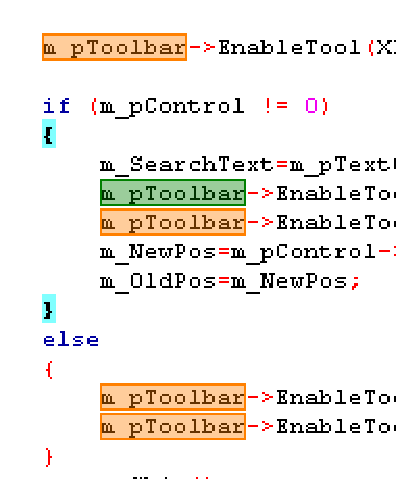
\includegraphics{incremental_search_example}

Wird der Suchbegriff in der aktiven Datei jedoch nicht gefunden, wird dies durch rotes Hinterlegen der Suchmaske signalisiert.

%- ESC now leaves IncSearch and optionally selects found phrase (if textcontrol has focus)
%- ALT-DELETE clears textcontrol (if it has the focus)
Die Icons in der Werkzeugleiste von Incremental Search sind wie folgt zu verstehen:

\begin{description}
\item[
\includegraphics{incremental_search_clear}] Löschen des Textes innerhalb der Suchmaske der Incremental Search Werkzeugleiste.
\item[
\includegraphics{incremental_search_previous},
\includegraphics{incremental_search_next}] Navigation zwischen den Vorkommen eines Suchbegriffes.
\item[
\includegraphics{incremental_search_highlight}] Dieser Knopf bewirkt, dass nicht nur der aktuelle gefundene Suchbegriff im Editor sondern auch weitere Vorkommnisse farblich hervorgehoben werden.
\item[
\includegraphics{incremental_search_selected}] Mit der Aktivierung dieser Option wird nur innerhalb eines selektierten Textes im Editor gesucht.
\item[
\includegraphics{incremental_search_matchcase}] Bewirkt, dass die Suche von Groß-/Kleinschreibung abhängt.
\end{description}

\hint{Die standardmäßigen Einstellungen dieser Werkzeugleiste sind in \menu{Settings,Editor,Incremental Search} konfigurierbar.}

\screenshot{incremental_search_settings}{Einstellungen für Incremental Search}
